In the same fashion as for the basic distance, here are the distances computed between the subset of articles and each year of the corpus:
\begin{figure}[H]
    \begin{minipage}[b]{0.3\linewidth}
        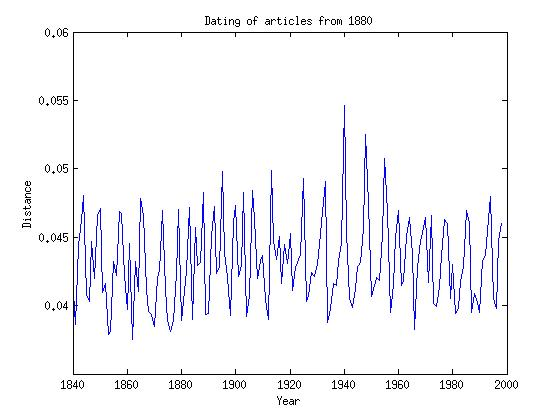
\includegraphics[scale=0.25]{Pictures/date_articles/chi2/dating1880.jpg}
        \caption{Dating articles from 1880 with the chi-square distance. Prediction is 1890}
    \end{minipage}\hfill
    \begin{minipage}[b]{0.3\linewidth}
        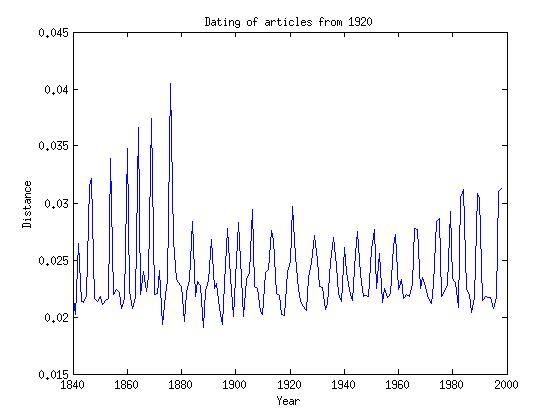
\includegraphics[scale=0.25]{Pictures/date_articles/chi2/dating1920.jpg}
        \caption{Dating articles from 1920 with the chi-square distance. Prediction is 1904.}
    \end{minipage}\hfill
    \begin{minipage}[b]{0.3\linewidth}
	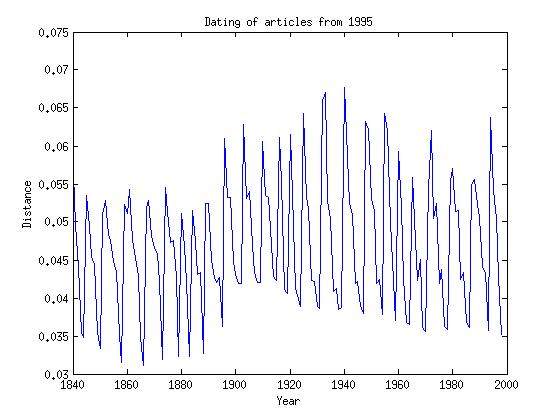
\includegraphics[scale=0.25]{Pictures/date_articles/chi2/dating1995_corrected.jpg}
        \caption{Dating articles from 1995 with the chi-square distance. Prediction is 1858.}
        \label{date_chi2}
    \end{minipage}
\end{figure}
With the \emph{Chi-Square} metric, the distances also look relatively random and there is again no evident prediction in these examples.